\subsubsection{Dilatação}

\begin{example}
  Compare os gráficos das funções reais $f, g , h: \R \to \R$ tais que:
  \begin{itemize}
    \item $f(x) = \sen x$;
    \item $g(x) = \frac 1 2 \cdot f(x)  = \frac 1 2 \cdot \sen x $;
    \item $h(x)= f(2 \cdot x)= \sen (2 \cdot x)$.
  \end{itemize}

  \begin{center}
    

\tikzset{every picture/.style={line width=0.75pt}} %set default line width to 0.75pt        

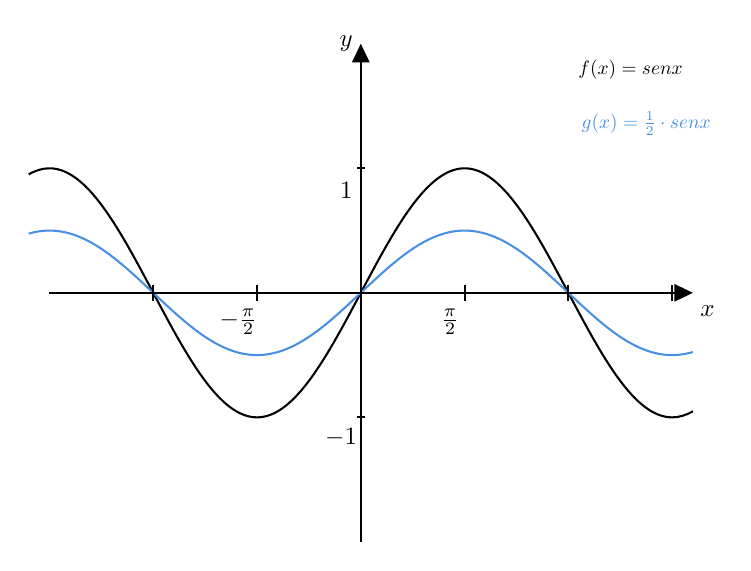
\begin{tikzpicture}[x=0.75pt,y=0.75pt,yscale=-1,xscale=1]
%uncomment if require: \path (0,300); %set diagram left start at 0, and has height of 300

%Shape: Wave [id:dp94416819522044] 
\draw   (180,102.94) .. controls (183.26,101.04) and (186.58,100) .. (190,100) .. controls (208.1,100) and (223.69,129.26) .. (240,160) .. controls (256.31,190.74) and (271.9,220) .. (290,220) .. controls (308.1,220) and (323.69,190.74) .. (340,160) .. controls (356.31,129.26) and (371.9,100) .. (390,100) .. controls (408.1,100) and (423.69,129.26) .. (440,160) .. controls (456.31,190.74) and (471.9,220) .. (490,220) .. controls (493.42,220) and (496.74,218.96) .. (500,217.06) ;
%Shape: Wave [id:dp05495114548578883] 
\draw  [color={rgb, 255:red, 74; green, 144; blue, 226 }  ,draw opacity=1 ] (180,131.47) .. controls (183.26,130.52) and (186.58,130) .. (190,130) .. controls (208.1,130) and (223.69,144.63) .. (240,160) .. controls (256.31,175.37) and (271.9,190) .. (290,190) .. controls (308.1,190) and (323.69,175.37) .. (340,160) .. controls (356.31,144.63) and (371.9,130) .. (390,130) .. controls (408.1,130) and (423.69,144.63) .. (440,160) .. controls (456.31,175.37) and (471.9,190) .. (490,190) .. controls (493.42,190) and (496.74,189.48) .. (500,188.53) ;
%Straight Lines [id:da13690129851328403] 
\draw    (190,160) -- (498,160) (240,156) -- (240,164)(290,156) -- (290,164)(340,156) -- (340,164)(390,156) -- (390,164)(440,156) -- (440,164)(490,156) -- (490,164) ;
\draw [shift={(500,160)}, rotate = 180] [fill={rgb, 255:red, 0; green, 0; blue, 0 }  ][line width=0.75]  [draw opacity=0] (8.93,-4.29) -- (0,0) -- (8.93,4.29) -- cycle    ;

%Straight Lines [id:da021329477973490496] 
\draw    (340,280) -- (340,42) (338,220) -- (342,220)(338,160) -- (342,160)(338,100) -- (342,100) ;
\draw [shift={(340,40)}, rotate = 450] [fill={rgb, 255:red, 0; green, 0; blue, 0 }  ][line width=0.75]  [draw opacity=0] (8.93,-4.29) -- (0,0) -- (8.93,4.29) -- cycle    ;


% Text Node
\draw (470,52.5) node [scale=0.7]  {$f( x) =senx$};
% Text Node
\draw (383,174) node [scale=0.9,color={rgb, 255:red, 0; green, 0; blue, 0 }  ,opacity=1 ]  {$\frac{\pi }{2}$};
% Text Node
\draw (281,174) node [scale=0.9,color={rgb, 255:red, 0; green, 0; blue, 0 }  ,opacity=1 ]  {$-\frac{\pi }{2}$};
% Text Node
\draw (333,110.5) node [scale=0.9]  {$1$};
% Text Node
\draw (330.5,229.5) node [scale=0.9]  {$-1$};
% Text Node
\draw (477.5,78.5) node [scale=0.7,color={rgb, 255:red, 74; green, 144; blue, 226 }  ,opacity=1 ]  {$g( x) =\frac{1}{2} \cdot senx$};
% Text Node
\draw (507,169) node [scale=0.9]  {$x$};
% Text Node
\draw (333,40) node [scale=0.9]  {$y$};


\end{tikzpicture}

  \end{center}
  \begin{center}
    

\tikzset{every picture/.style={line width=0.75pt}} %set default line width to 0.75pt        

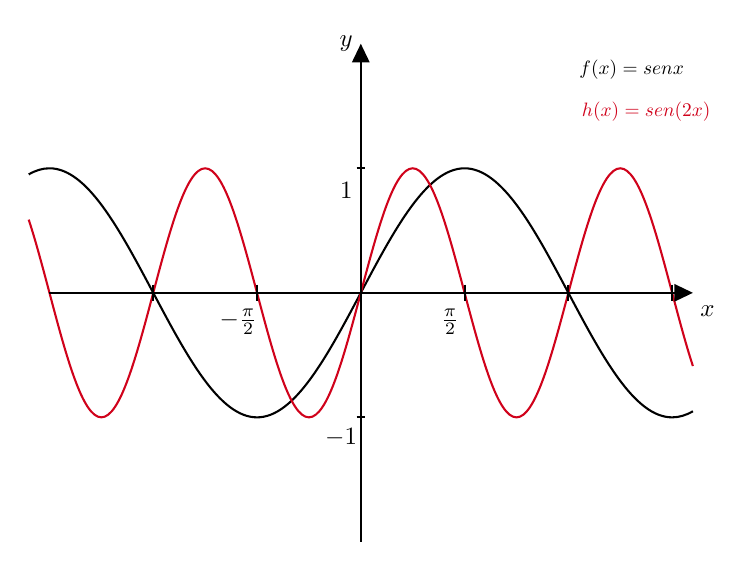
\begin{tikzpicture}[x=0.75pt,y=0.75pt,yscale=-1,xscale=1]
%uncomment if require: \path (0,300); %set diagram left start at 0, and has height of 300

%Shape: Wave [id:dp94416819522044] 
\draw   (180,102.94) .. controls (183.26,101.04) and (186.58,100) .. (190,100) .. controls (208.1,100) and (223.69,129.26) .. (240,160) .. controls (256.31,190.74) and (271.9,220) .. (290,220) .. controls (308.1,220) and (323.69,190.74) .. (340,160) .. controls (356.31,129.26) and (371.9,100) .. (390,100) .. controls (408.1,100) and (423.69,129.26) .. (440,160) .. controls (456.31,190.74) and (471.9,220) .. (490,220) .. controls (493.42,220) and (496.74,218.96) .. (500,217.06) ;
%Shape: Wave [id:dp05495114548578883] 
\draw  [color={rgb, 255:red, 208; green, 2; blue, 27 }  ,draw opacity=1 ] (180,124.73) .. controls (183.35,134.95) and (186.64,147.35) .. (190,160) .. controls (198.15,190.74) and (205.95,220) .. (215,220) .. controls (224.05,220) and (231.85,190.74) .. (240,160) .. controls (248.15,129.26) and (255.95,100) .. (265,100) .. controls (274.05,100) and (281.85,129.26) .. (290,160) .. controls (298.15,190.74) and (305.95,220) .. (315,220) .. controls (324.05,220) and (331.85,190.74) .. (340,160) .. controls (348.15,129.26) and (355.95,100) .. (365,100) .. controls (374.05,100) and (381.85,129.26) .. (390,160) .. controls (398.15,190.74) and (405.95,220) .. (415,220) .. controls (424.05,220) and (431.85,190.74) .. (440,160) .. controls (448.15,129.26) and (455.95,100) .. (465,100) .. controls (474.05,100) and (481.85,129.26) .. (490,160) .. controls (493.36,172.65) and (496.65,185.05) .. (500,195.27) ;
%Straight Lines [id:da13690129851328403] 
\draw    (190,160) -- (498,160) (240,156) -- (240,164)(290,156) -- (290,164)(340,156) -- (340,164)(390,156) -- (390,164)(440,156) -- (440,164)(490,156) -- (490,164) ;
\draw [shift={(500,160)}, rotate = 180] [fill={rgb, 255:red, 0; green, 0; blue, 0 }  ][line width=0.75]  [draw opacity=0] (8.93,-4.29) -- (0,0) -- (8.93,4.29) -- cycle    ;

%Straight Lines [id:da021329477973490496] 
\draw    (340,280) -- (340,42) (338,220) -- (342,220)(338,160) -- (342,160)(338,100) -- (342,100) ;
\draw [shift={(340,40)}, rotate = 450] [fill={rgb, 255:red, 0; green, 0; blue, 0 }  ][line width=0.75]  [draw opacity=0] (8.93,-4.29) -- (0,0) -- (8.93,4.29) -- cycle    ;


% Text Node
\draw (470.5,52.5) node [scale=0.7]  {$f( x) =senx$};
% Text Node
\draw (383,174) node [scale=0.9,color={rgb, 255:red, 0; green, 0; blue, 0 }  ,opacity=1 ]  {$\frac{\pi }{2}$};
% Text Node
\draw (281,174) node [scale=0.9,color={rgb, 255:red, 0; green, 0; blue, 0 }  ,opacity=1 ]  {$-\frac{\pi }{2}$};
% Text Node
\draw (333,110.5) node [scale=0.9]  {$1$};
% Text Node
\draw (330.5,229.5) node [scale=0.9]  {$-1$};
% Text Node
\draw (477.5,72.5) node [scale=0.7,color={rgb, 255:red, 208; green, 2; blue, 27 }  ,opacity=1 ]  {$h( x) =sen( 2x)$};
% Text Node
\draw (507,169) node [scale=0.9]  {$x$};
% Text Node
\draw (333,40) node [scale=0.9]  {$y$};


\end{tikzpicture}

  \end{center}
\end{example}

\begin{example}
Compare os gráficos das funções reais $f, g , h: \R \to \R$ tais que
$f(x) = \sen x$, \\ $g(x) = -1 \cdot f(x)  = -1 \cdot \sen x $ , \\
$h(x)= f(-1 \cdot x)= \sen (-1 \cdot x)$.
\end{example}

Dessa forma, se a função real $g$ é tal que $g(x) = c \cdot f(d
\cdot x)$, então o gráfico de $g$ pode ser obtido, do gráfico de
$f$, através de uma dilatação horizontal determinada pelo parâmetro
$d$, e uma dilatação vertical determinada pelo parâmetro $c$. Se o
parâmetro for negativo, haverá, também, uma reflexão.
\begin{itemize}
  \item A dilatação vertical será:
        \begin{itemize}
          \item Um esticamento se $c>1$;
          \item Um encolhimento se $0<c<1$;
          \item Um esticamento composto com reflexão em relação ao eixo $x$ se $c<-1$;
          \item Um encolhimento composto com reflexão em relação ao eixo $x$ se
          $-1<c<0$.
        \end{itemize}
  \item A dilatação horizontal será:
        \begin{itemize}
          \item Um encolhimento se $d>1$;
          \item Um esticamento se $0<d<1$;
          \item Um encolhimento composto com reflexão em relação ao eixo $y$ se $d<-1$;
          \item Um esticamento composto com reflexão em relação ao eixo $y$ se
          $-1<d<0$.
        \end{itemize}
\end{itemize}

\begin{onlineact}
    \khan{https://pt.khanacademy.org/math/algebra2/manipulating-functions/shifting-functions/e/shift-functions}
    {Deslocamento de Funções}.
\end{onlineact}

\begin{onlineact}
    \khan{https://pt.khanacademy.org/math/algebra2/manipulating-functions/stretching-functions/e/shifting_and_reflecting_functions}
    {Como Transformar Funções}.
\end{onlineact}